\section{Experiments}
\label{sec:experiments}

% \begin{description}
% 	\item [RNN] 10, 25, 50, 75, and 100 gated recurrent units.
% 	\item [Training] 200 epochs.
% 	\item [Learning curves] cost functions, accuracies, and some metric for weights.
% 	\item[Activations] of GRUs for tunes.
% 	\item[Evaluation] on test set as a table.
% 	\item [Reconstructions] of test examples.
% \end{description}

The experiments were run for model 1, the normal RNN model using only original input and model 2, the extended RNN model using the previous prediction step output as input to the next step.

They are implemented in Python with the Theano and Lasagne library, using mini-batch gradient descent with the ADAM optimizer \cite{Kingma2014c}.  

\subsection{Regularization} % (fold)
\label{sub:regularization}

Dropout of 20\% or 50\% was applied right before the GRU layer in the input network. By dropping out notes along the melodies, a lossy noise and therefore a completion task is introduced to the models, so during training the next-step prediction will rely more on the previous GRU activations $\vec{h}\idx{t-1}$ and the horizontal connections will be enhanced to make up for the missing input. The stronger horizontal connections will hopefully combine some more general musical rules and therefore reduce overfitting. 

An $L_2$-regularization term is also added to the total cost during training for reducing overfitting.
% subsection regularization (end)


\subsection{Evaluation}

The prediction accuracy and categorical cross entropy for both classes are recorded for each epoch and seen in the learning curves in Figure \ref{fig:learning_curves}.

To investigate the connections in the GRU layer, the mean, Frobenius norm and positive value fractions of horizontal and vertical weights, where the trend in the overall magnitude and sign of the weights are expected to be seen. \\ \\

The two models with and without dropout and/or regularization are tested for 10, 25, 50, 75, and 100 gated recurrent units, so scaling of performance can be investigated and the effect of the regularization methods compared. The scaling of performance with the number of GRU are clearly seen, but not shown here, so 100 GRU are used as a standard and for these regularization methods and model architectures can be compared in Table \ref{tab:test_eval}.

All models were trained for 200 epochs, as they reaches convergence after 150 epochs in the learning curves seen in Figure \ref{fig:learning_curves}\\ \\

\subsection{Reconstructions}

After training, the models were evaluated on 2 test songs, handpicked out of the unseen test set. The notes in the original melody (input) are highlighted by colors corresponding to the GRU activations, so patterns, like scale and rhythmical motifs, leading to higher activation can be localized and the functionality of the GRU identified.

To investigate the distribution of the pitch and duration classes, the frequencies of each class in the original data are represented in a histogram in Figure~\ref{fig:histogram}

All reconstructions can be translated back to the \texttt{music21} format, written to a midi file, played, written as a musical score and compared against the original melody.

\begin{table*}
    \centering
    \caption{
        The test evaluation measures.
    }
    \label{tab:test_eval}
    % \setlength{\tabcolsep}{1em}
    \sisetup{
        table-number-alignment = center
    }
    \begin{tabular}{
            l@{}
            S[table-format = 1.0]
            S[table-format = 0.2]
            S[table-format = 1.0]
            S[table-format = 1.3]
            S[table-format = 1.3]
            S[table-format = 2.2]
            S[table-format = 2.2]
        }
        \toprule
        & {Model} 
        & {$p\idx{dropout}$}
        & {$\alpha_2$}
        & {$L\idx{pitch}$}
        & {$L\idx{duration}$}
        & {$A\idx{pitch}$(\%)}
        & {$A\idx{duration}$(\%)} \\
        \midrule
        \input{../data/eval_table}
        \bottomrule
    \end{tabular}
\end{table*}

\begin{figure*}
    \centering
    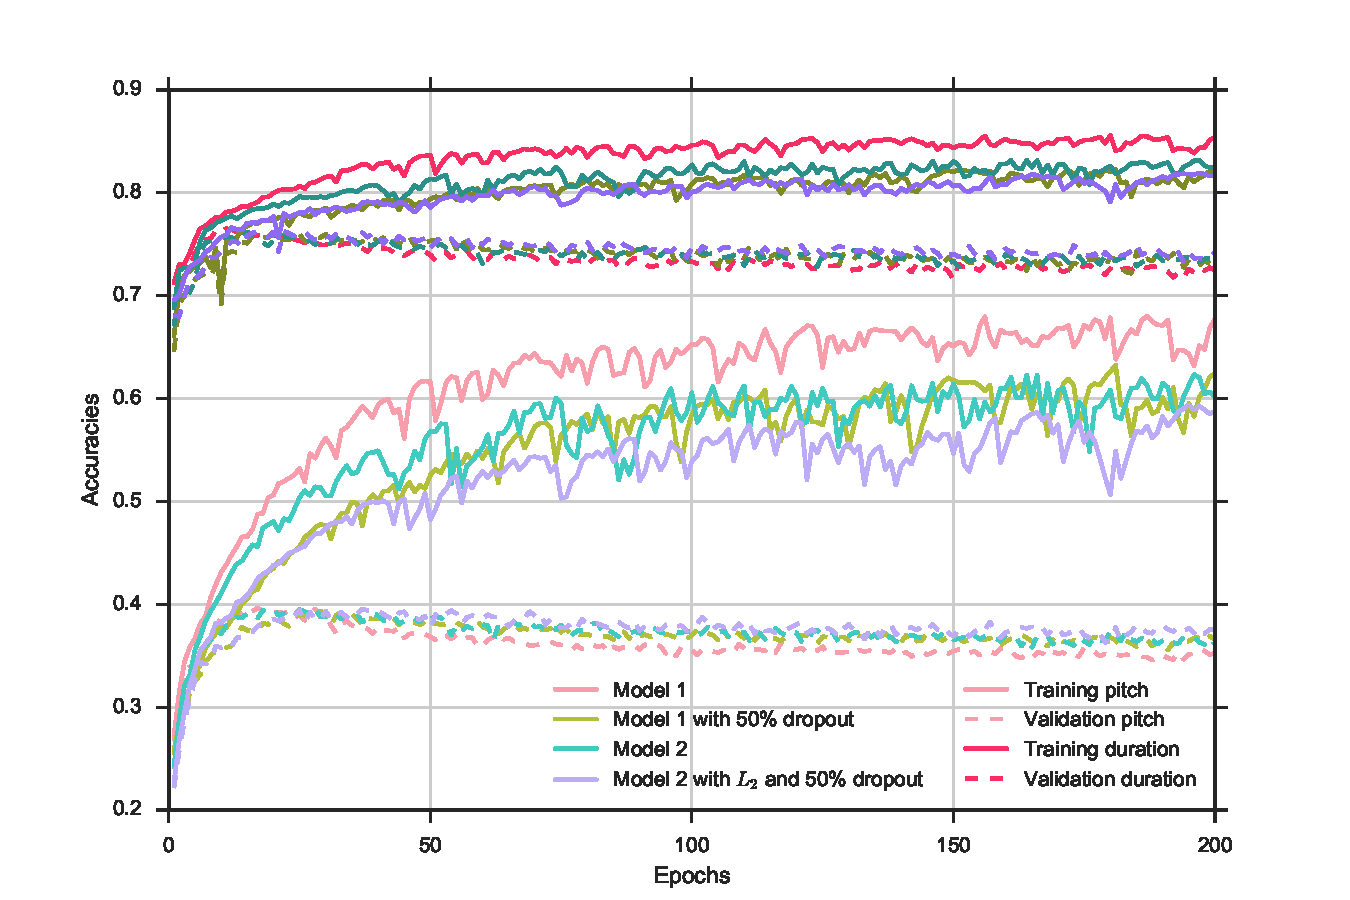
\includegraphics[width = .80\linewidth]{acc_learning_curves}
    \caption{Learning curves over next-step prediction accuracies for both model types with and without regularization. The models are evaluated on both training (solid lines) and validation sets (dashed lines) for pitch (turquoise) and duration classes (orange).}
    \label{fig:learning_curves}
\end{figure*}

% \begin{figure*}
%     \centering
% 	\hspace*{\fill}
%     \subbottom[\label{fig:learning_curves:type1}]{
%         \includegraphics[width = .45\linewidth]{model_1_gru_100_bs_10_e_200_acc}
%     }
%     \hfill
%     \subbottom[\label{fig:learning_curves:type2}]{
%         \includegraphics[width = .45\linewidth]{model2_gru_100_bs_10_e_200_acc}
%     }
% 	\hspace*{\fill}
%     \caption{Learning curves over next-step prediction accuracies for \subcaptionref{fig:learning_curves:type1} model type 1 and \subcaptionref{fig:learning_curves:type2} model type 2 without any regularization. The models are evaluated on both training (solid lines) and validation sets (dashed lines) and for pitch (turquoise) and duration classes (orange).)
%     }
%     \label{fig:learning_curves}
% \end{figure*}

% \begin{figure*}
%     \centering
% 	\hspace*{\fill}
%     \subbottom[\label{fig:learning_curves_regularized:type1}]{
%         \includegraphics[width = .45\linewidth]{model2_with_50p_dropout_gru_100_bs_10_e_200_acc.pdf}
%     }
%     \hfill
%     \subbottom[\label{fig:learning_curves_regularized:type2}]{
%         \includegraphics[width = .45\linewidth]{model_1_with_50p_dropout_gru_100_bs_10_e_200_acc}
%     }
% 	\hspace*{\fill}
%     \caption{Learning curves over next-step prediction accuracies for \subcaptionref{fig:learning_curves_regularized:type1} model type 1 and \subcaptionref{fig:learning_curves_regularized:type2} model type 2, both with $50\%$ dropout. The models are evaluated on both training (solid lines) and validation sets (dashed lines) and for pitch (turquoise) and duration classes (orange).
%     }
%     \label{fig:learning_curves_regularized}
% \end{figure*}


% \begin{figure*}
%     \centering
%     \setkeys{Gin}{height=.28\textheight}
% 	\hspace*{\fill}
%     \subbottom[\label{fig:histogram_orig:pitch}]{
%         \includegraphics{orig_pitch_freq_barplot}
%     }
%     \hfill
%     \subbottom[\label{fig:histogram_orig:duration}]{
%         \includegraphics{orig_duration_freq_barplot}
%     }
% 	\hspace*{\fill}
%     \caption{Histograms showing statistical frequency of pitch \subcaptionref{fig:histogram_orig:pitch} and duration \subcaptionref{fig:histogram_orig:duration} classes.)
%     }
%     \label{fig:histogram_orig}
% \end{figure*}

\begin{figure*}
    \centering
    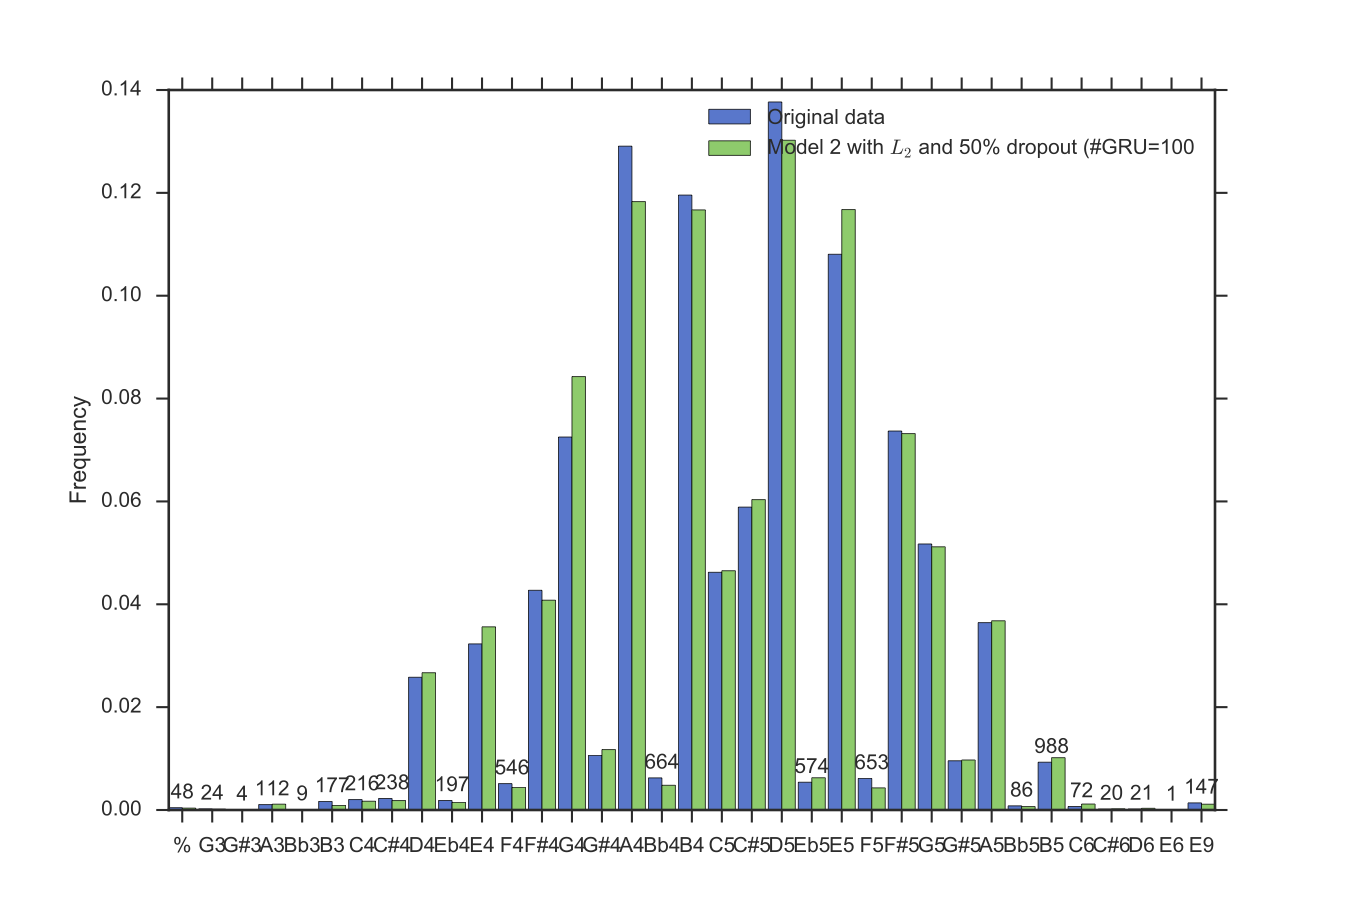
\includegraphics[width=.8\textwidth]{models_pitch_freq_barplot}
    \caption{Histograms showing statistical frequency of pitch classes in the (blue) original data and in the (green) reconstructions produced by model type 2 with dropout of 50\% and $L_2$-regularization.}
    \label{fig:histogram}
\end{figure*}
